% !TEX root = main.tex

\chapter{Experimental results}
\label{ch:results}
This chapter collects the key experimental results obtained during my master's work:
\begin{itemize}
\item Section \ref{sec:resultaod} contains the characterization of the AOD.
\item In Section \ref{sec:fullsetup} the characterization of the test setup is presented. Polarization, stability, and focus spot have been checked. In particular, two methods have been used to measure a $\mu$m focus spot: razor blade scans, and small pixel size camera.
\item In Section \ref{sec:finalsetup} the results from experiments with trapped ions are presented. First, single-qubit manipulation via Ramsey interferometry, which also allowed for a check of addressing performance. Second, a cQED experiment where single photons were generated from a single ion in a string, via a cavity-mediated Raman process (Section \ref{sec:ramanprocess}).
\end{itemize}
\section{AOD}
\label{sec:resultaod}
The two main parameters we are interested here are the diffraction efficiency and the response time. For the diffraction efficiency we measured the total output power of the light $P_{tot}$ and then the power of the first diffracted order $P_{1}$. Diffraction efficiency is defined as the ratio between the two
\begin{equation}
\label{eq:de}
\text{DE} = \frac{P_1}{P_{tot}}.
\end{equation}
The response time is the time it takes for the light to move to a new position corresponding to an RF frequency change. The measurement of the response time gives us an idea of how long it takes to switch from one ion to the other.\par
Before measuring the diffraction, the optimal RF power to drive the AOD has been found by maximizing the power of the first diffracted order with the AOD set at its central frequency. Power measurements of the light were done with a Thorlabs PM100D, and the AOD was driven with an amplifier and an RF signal generator. The highest efficiency at the central frequency was found for an RF power of 0.11 W, and for the rest of the measurements it was kept at that value. Furthermore, to optimize the linear input polarization, a PBS followed by a half-waveplate were placed before the AOD, the waveplate was rotated to maximize the power of the diffracted light. In Figure \ref{DE} a plot of the measured diffraction efficiency as a function of the RF frequency is displayed. Within a bandwidth of 50 MHz from 105 MHz to 155 MHz, we can see that more than 70 \% of the light is in the first diffracted order as expected from the datasheet (Appendix \ref{sec:aoddata}), even though the bandwidth looks shifted with respected to the nominal central frequency of 120 MHz.\par
In order to measure the response time, a voltage controlled oscillator (VCO) was used to generate the RF signal. The VCO was supplied a square wave that alternated between two voltages corresponding to two different frequencies $\sim 96$ and $\sim 127$ MHz. The laser light diffracted into the -1 order was measured with a photodiode. The photodiode was aligned with the light at one particular frequency, such that when the light moves, the beam would not hit the diode and the signal generated changes. In Figure \ref{response}, the signal of the photodiode, together with the supplied VCO signal are plotted. Response time is $\sim 8\,\mu$s, with $3\,\mu$s delay and $5\,\mu$s rise time. From the beam diameter (2.14 mm, $1/e^2$ of intensity) and the acoustic velocity in the crystal (0.65 mm/$\mu$s, Appendix \ref{sec:aoddata}) we expect $4.9$ $\mu$s rise time, while the delay indicates that the distance between the piezo and the edge of the beam is 1.95 mm.

\begin{figure}
\centering
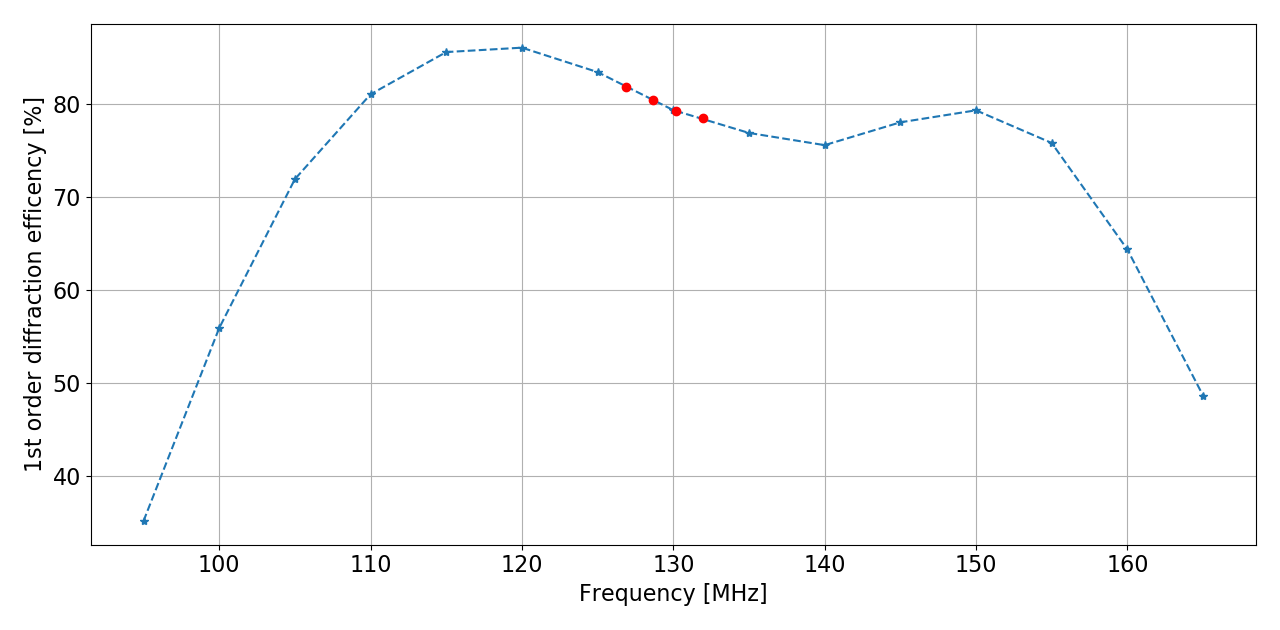
\includegraphics[width = .95\textwidth]{DE2}
\caption{Measurement of the diffraction efficiency of the AOD as a function of the RF driving frequency (Equation \eqref{eq:de}). Blu stars indicate the measured points. Red points indicate the expected frequencies associated with addressing 4 ions for an axial COM frequency of 780 kHz (the conditions for the experiment presented in Section \ref{sec:singlequbitmanipulation}), the theoretical separations are 5.15 $\mu$m for the two outer ions, and 4.77 $\mu$m for the inner ions.}
\label{DE}
\end{figure}

\begin{figure}
\centering
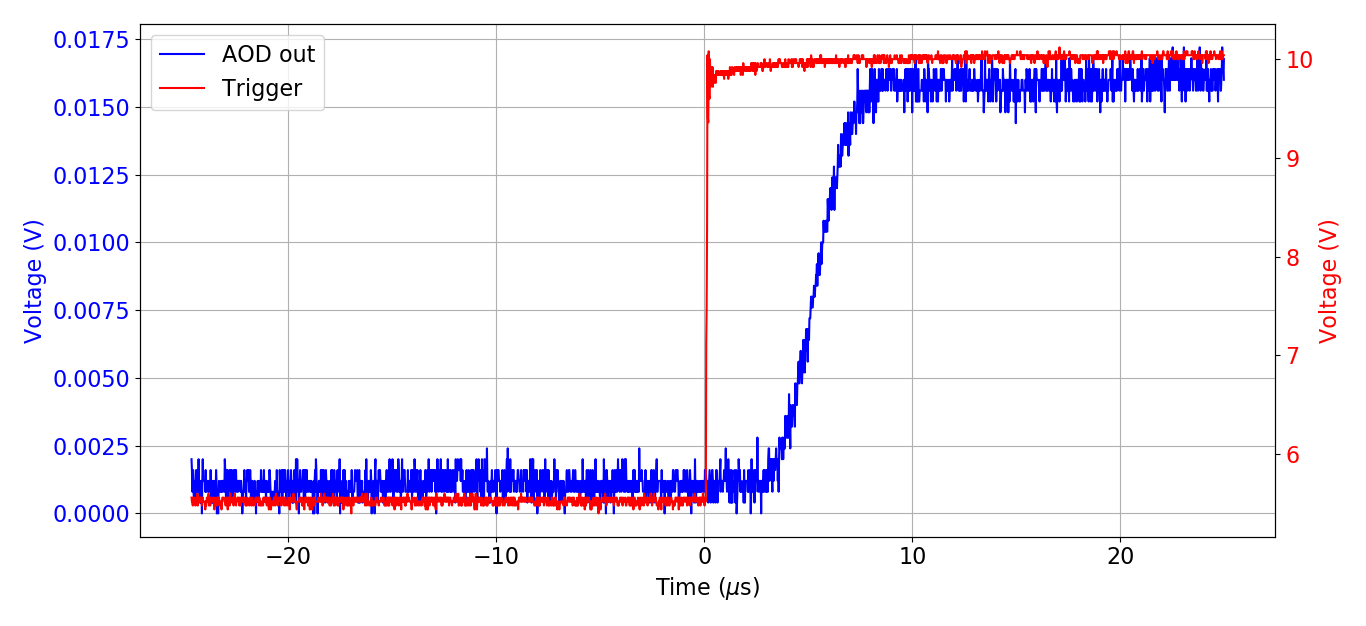
\includegraphics[width = .95\textwidth]{response}
\caption{Measured response time of the AOD, plotted are the photodiode signal in blue on the left $y$ axis, and the VCO voltage is in red on the right axis. The voltage of the VCO determines the frequency of the RF sent to the AOD. The change here corresponds to a frequency shift of $\sim$31 MHz between $\sim 96$ and $\sim 127$ MHz. At the highest voltage, the photodiode measures the -1st diffracted light.}
\label{response}
\end{figure}

\section{Full test setup characterization}
\label{sec:fullsetup}
The test setup was built on an optical table with a spare objective since the one installed in the vacuum chamber was already in use for ion imaging. The layout of the system in Figure \ref{addressingsetup} was replicated.

\subsection{Waist: Knife-Edge method}
\label{sec:knifeedge}
\begin{figure}[H]
\centering
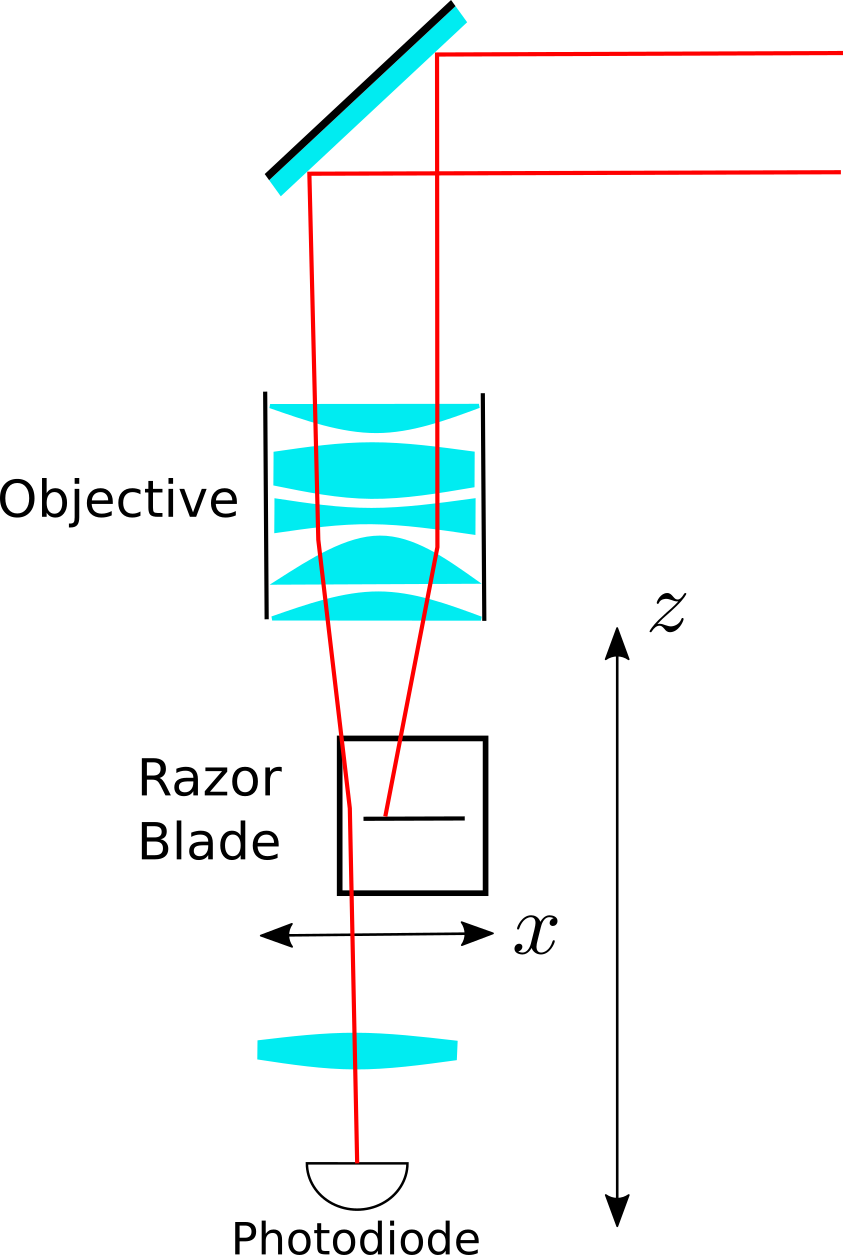
\includegraphics[scale = 1.1]{razorsetup}
\caption{Scheme of the razor scan. A translation stage allows for moving the blade in the direction x, perpendicular to the beam, and z, along the beam.}
\label{razorscan}
\end{figure}
Measuring a micrometer scale waist is not an easy task, the first method applied consisted of mounting a razor blade on a translational stage. The setup used is showed in Figure \ref{razorscan}, after the objective the blade is present, and since the beam is quickly diverging after the focus, a lens is used to refocus the light into a photodiode. The stage is moved in the $x$ direction cutting the beam perpendicularly such that the blade is scanning the beam profile. A filter was inserted in order to not saturate the photodiode.
In the $z$ direction the stage was controlled with a manual screw with resolution of $1\,\mu$m. While in the $x$ direction, the stage had to be moved with sub-micrometer precision, so instead there was a piezo actuator controlled by custom software. The same software also controlled a multimeter that measured the voltage of the photodiode. To get the profile $W(z)$ (Equation \eqref{waistprofile}) of the beam, the measurement procedure was as follows
\begin{itemize}
\item Position blade at desired $z$ coordinate
\item Scan beam in $x$ direction with blade
\item Shift $z$ direction
\end{itemize}
The procedure is repeated for sufficient values of $z$ to scan at least a few Raylegh ranges. The beam width can be calculated from the scans by fitting the data with equation (2) of \cite{knifeedge}. In Figure \ref{examplerazorscan} we report an example of a scan that gave a minimal waist. The errorbars come from statistical average, every data point is a mean over 5 measurements, and the error is the standard deviation. The fit in this case gave a width $W$ (beam width $1/e^2$) of $3.47\pm 0.06\,\mu$m, the smallest width obtained with this method, but significantly broader than the 1 $\mu$m simulated waist. Furthermore, the profile $W(z)$ was not symmetric and could not be fitted with Equation \eqref{waistprofile}. A possible explanation is that with this commercially-available razor blade, the accuracy is limited by the positioner and the blade roughness. The latter was not known at the few micrometer scale of the beam waist. In comparison, authors of \cite{Cannon:86} have used, instead of a common razor blade, a glass substrate etched with an effective knife-edge features with which they were able to measure a 1 $\mu$m waist.
\begin{figure}
\centering
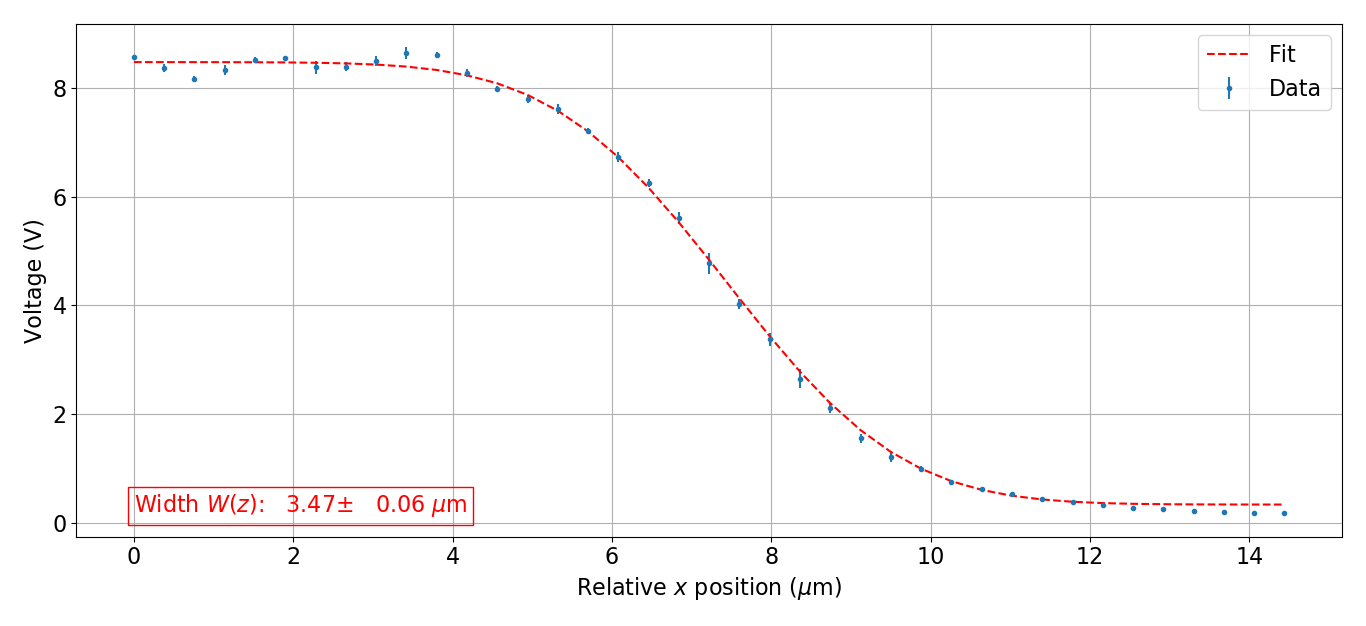
\includegraphics[width=1\textwidth]{img/razorscan}
\caption{Razor scan at the waist of the beam $z=0$}
\label{examplerazorscan}
\end{figure}


\subsection{Waist: Camera}
\label{waistcamera}
Since the Knife-Edge method did not prove that we had achieved our desired waist, a  more direct approach has been subsequently adopted. We measured directly the beam with a camera from IDS model UI-1490LE-M-GL. This camera has a pixel size of 1.67 $\mu$m with no spacing between pixels. It should therefore be suitable to measure a focus spot with a $\mu$m precision. A 1 $\mu$m focus should hit one single pixel, and if aligned between two pixels, a Gaussian profile could also be fitted.
In addition, unlike the Knife-Edge technique, a camera provides 2-dimensional information about the beam shape and can be exploited to look for aberrations in the system. The setup is almost the same as Figure \ref{razorscan}, but the camera now replaces the razor blade, and there is no need for scanning in the $x$ direction, as the $z$ is enough to reconstruct the profile $W(z)$. An additional filter was used to optimize the light reaching the camera in order to not saturate it.
% \begin{figure}
%      \centering
%      \begin{subfigure}[b]{0.67\textwidth}
%          \centering
%          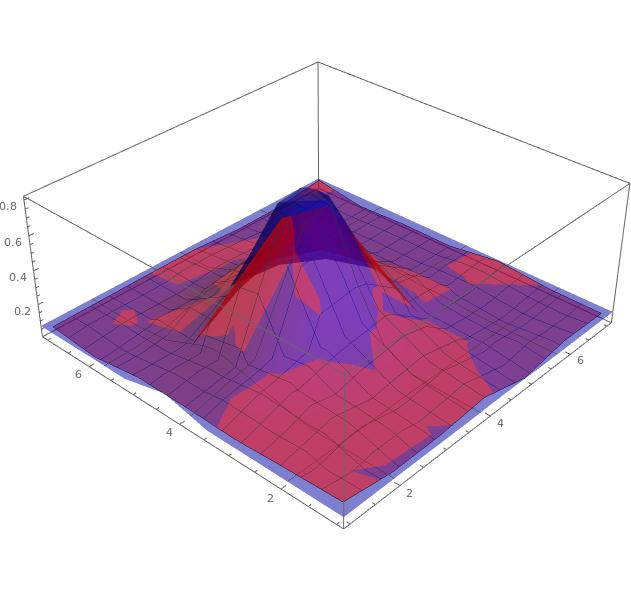
\includegraphics[width = \textwidth]{camera}
%           \caption{Fitted data from the camera. In red color, the normalized pixel value is displayed, while the blue curve is a fitted 2D Gaussian. On the axis there is the pixel number}
%      \end{subfigure}
%      \hfill
%      \begin{subfigure}[b]{0.3\textwidth}
%          \centering
%          
\includegraphics[width=\textwidth]{cameraoriginal}
%         \vspace{5em}
%          \caption{Original photo from the camera.}
%          %\label{fig:three sin x}
%
%      \end{subfigure}
%         \caption{}
%        \label{fig:camera}
% \end{figure}
For every desired $z$ displacement, a photo with the camera is taken, post processed, and then the camera is displaced to the new $z$ coordinate. Post processing is done by fitting the pixel values with a 2-dimensional Gaussian
\begin{equation}
P = A \exp\left\{-\frac{(x-x_0)^2}{2\sigma_x^2}\right\} \exp\left\{-\frac{(y-y_0)^2}{2\sigma_y^2} \right\}.
\end{equation}
The fit parameters are $A,x_0,y_0,\sigma_x,$ and $\sigma_y$. From the standard deviations $\sigma_x$ and $\sigma_y$ the beam width in the $x$ and $y$ direction at position $z$: $W_x(z),W_y(z)$ can be determined as $W_x(z) = 2\cdot 1.67\cdot \sigma_x$ and respectively $W_y(z) = 2\cdot 1.67\cdot \sigma_y$, where $1.67\,\mu$m is the pixel size (see caption of Figure \ref{gauss}). The full profiles $W_x(z)$ and $W_{y}(z)$ can be found in Figure \ref{cameraprofile}. Here anomalies can be noticed. The profile is asymmetric and does not follow Equation \ref{waistprofile}, nonetheless a width $<2.5\,\mu$m has been measured. We decided to install the system and measure more accurately the waist with a single ion.
\begin{figure}
\centering
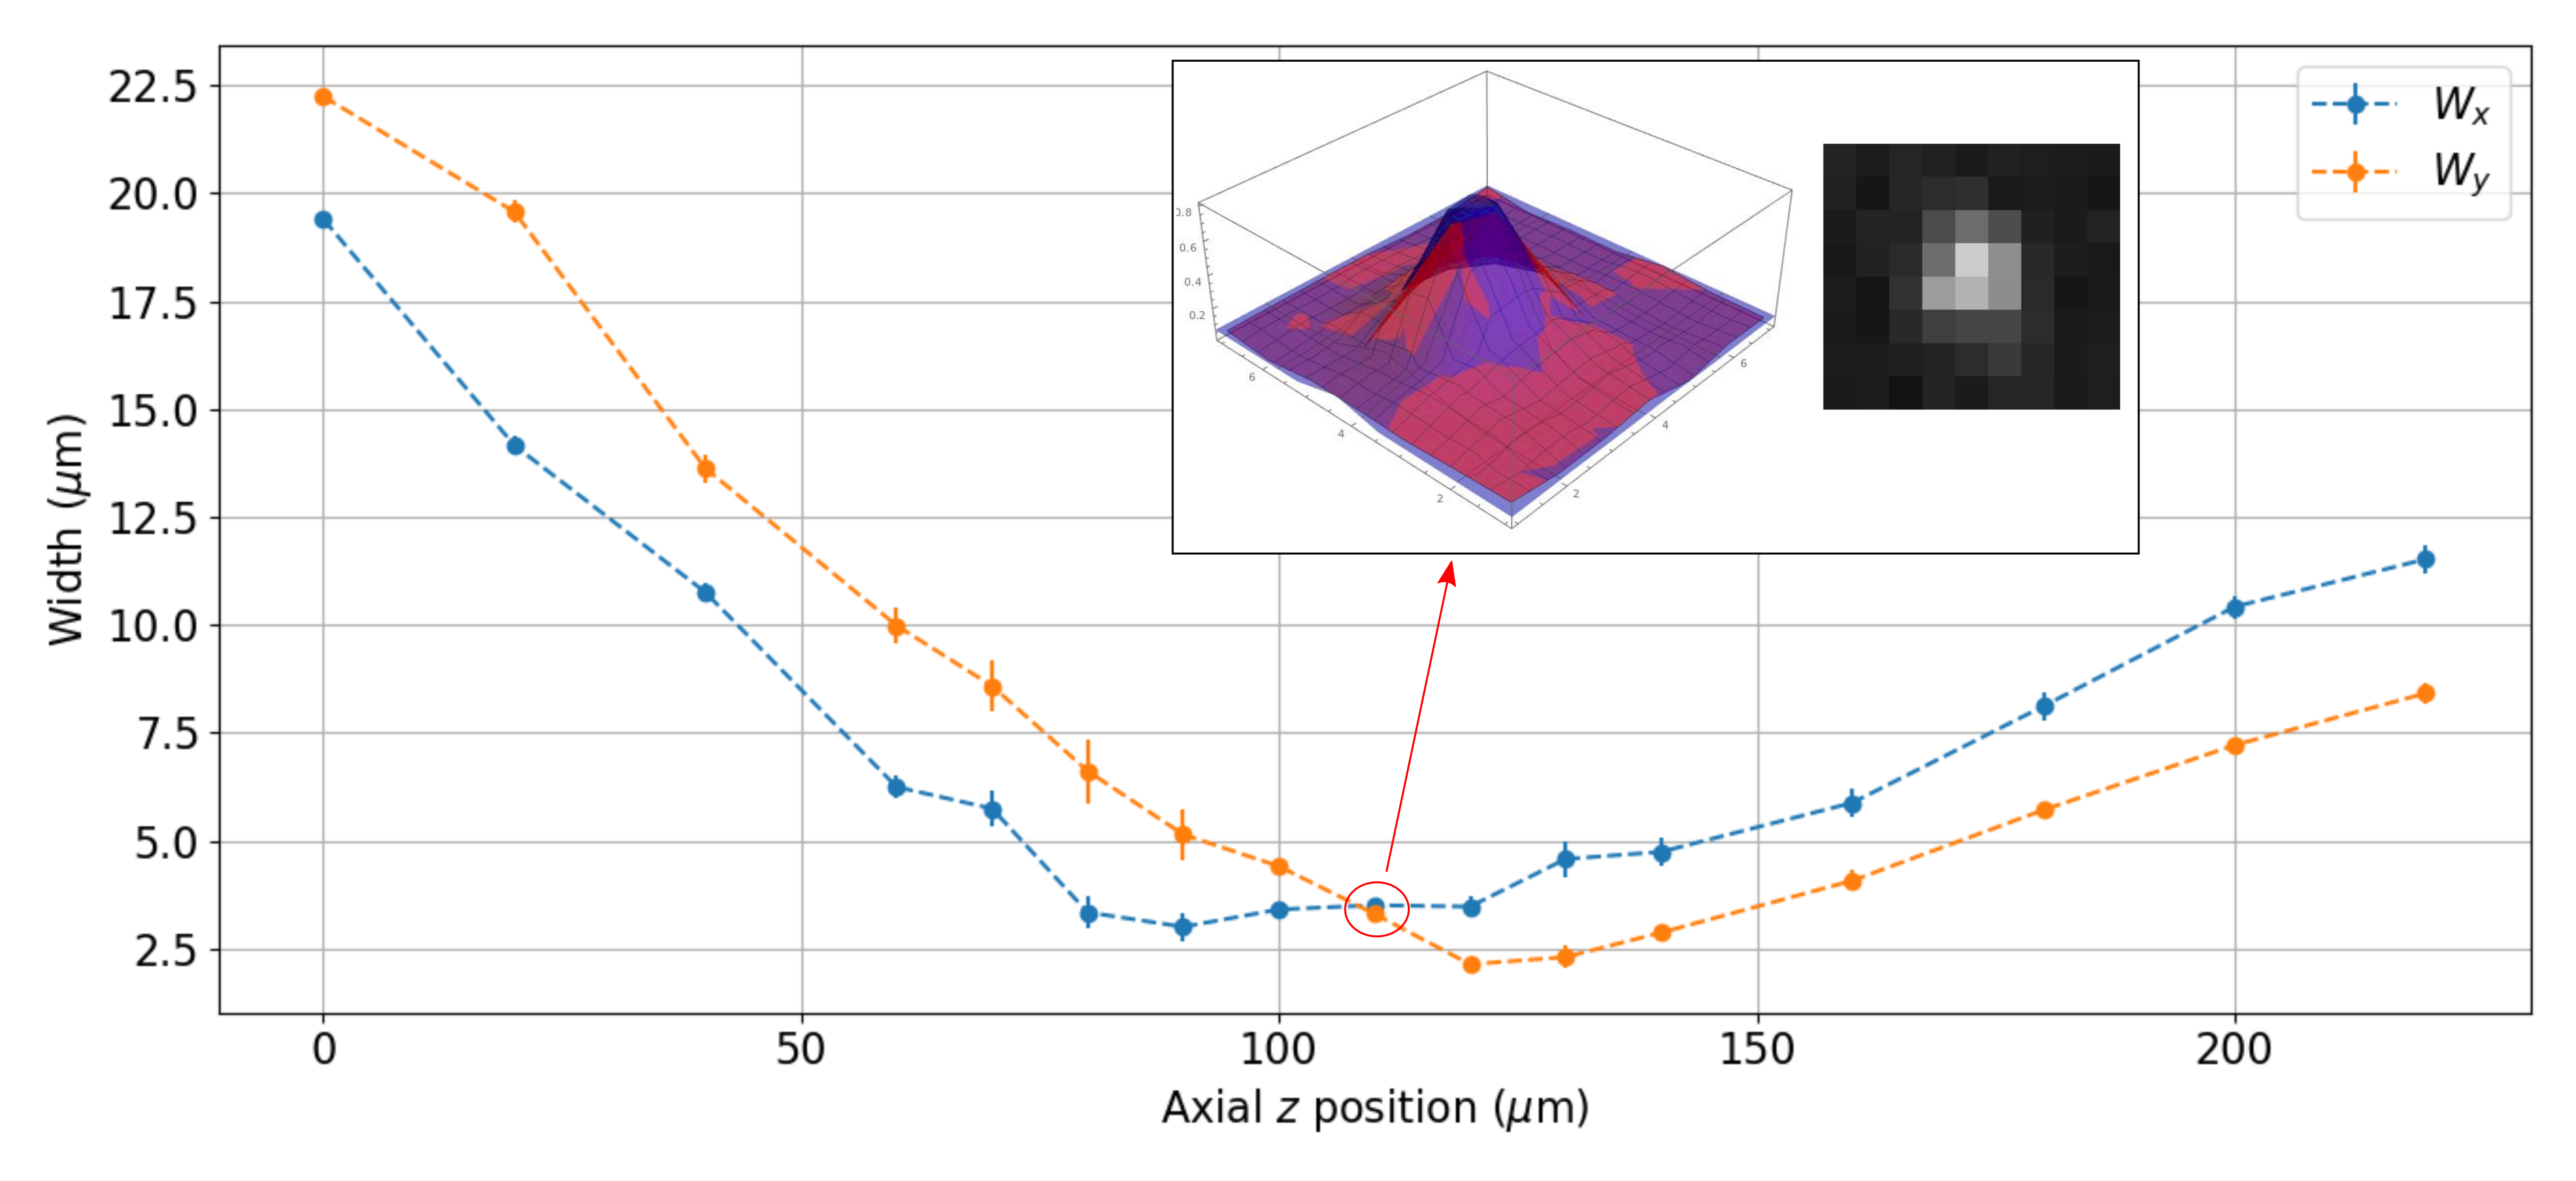
\includegraphics[width=1\textwidth]{cameraprofile_inset}
\caption{Profile of the Gaussian beam along $z$ measured with the IDS camera. Errorbars are estimated from fit. In the inset an example of raw data and Gaussian fit. In red color, the normalized pixel value is displayed, while the blue curve is a fitted 2D Gaussian. On the axis there is the pixel number.}
\label{cameraprofile}
\end{figure}

\subsection{Polarization}
\label{sec:polarization}
As discussed in the design Section \ref{sec:addressing} and in the Raman process \ref{sec:ramanprocess}, polarization is an important component as atomic transitions are polarization sensitive, thus the polarization capabilities of the system had to be tested. The goal is to allow for the generation of vertical, horizontal, left circular, and right circular polarization at the ion position and test how well they are achieved. Polarization can be changed with two plates: a half wave plate after the AOD, and a quarter wave plate right before the objective, see Figure \ref{addressingsetup}. In order to characterize the polarization at various points in the optical path of the addressing setup, the three Stokes parameters $S_i$ \cite{stokes} were measured with a polarimeter from Sc\"after + Kirchhoff series SK010PA.\par
Stokes parameters quantify the type of polarization of an electric field. Linear polarized light has Stokes parameters $S_2,S_3 = 0$, while $S_1 = \pm 1$ for horizontal and vertical polarization respectively. Circular polarized light has $S_1, S_2 = 0$ and $S_3=\pm 1$ for right hand and left hand circular polarization respectively.\par
The first step was to characterize the polarization after the waveplate after the AOD ($\lambda/2$, WP B, Figure \ref{addressingsetup}), the main result from this characterization is that horizontal polarization can be achieved immediately after WP B with an angle of $267.2\pm 0.1 ^{\circ}$, and vertical is achieved with an angle of $312.5\pm0.1^{\circ}$ obtained from fitting a sine on the first Stokes parameter. From the same fit, the semiperiod of the polarization is $45.3\pm 0.6^\circ$ consistent with the $45^\circ$ expected for a half waveplate.\par
Afterwards, we measured the polarization after the objective at the focus spot where the ions ideally sit. For this measurement we set the $\lambda/2$ WP B first at $267.2\pm 0.1^\circ$, and then at $312.5\pm0.1^{\circ}$, for both numbers we measured the three Stokes parameters as a function of the $\lambda/4$ angle. Results are summarized in table \ref{polarizationstable}, in appendix \ref{app:polarization} the full plots are reported.
\begin{table}
\centering
\begin{tabular}{c c c c c c}
 \toprule
    {Desired polarization} & {$\lambda/2$ WP B ($^\circ$)} & {$\lambda/4$ ($^\circ$)} & Stokes 1 & Stokes 2 & Stokes 3\\ \midrule\midrule
   Horizontal & $267.2\pm 0.1$ & $49.7\pm0.1$ & 1.00 & -0.01 & 0.01\\
   Vertical   & $312.5\pm0.1$ & $48.1\pm0.1$ &  0.96 &  0.12 & -0.26 \\ \midrule
   Right circular & $267.2\pm 0.1$ & $4\pm 0.1$ &  0.05 & -0.02 & 1.00 \\
   Right circular & $312.5\pm0.1$ & $93.1\pm0.1$ & 0.10 & 0.01 & 1.00  \\\midrule
  Left circular & $267.2\pm 0.1$ & $95.4\pm0.1$ &  0.06 & 0.01 & -1.00  \\
    Left circular & $312.5\pm0.1$  & $3.1\pm0.1$ &  -0.20 & 0.06 & -0.98  \\ \bottomrule
\end{tabular}
\caption{Desired polarization at the ion position and angles of the waveplates $\lambda/2$ WP B and $\lambda/4$ (Ref. Figure \ref{addressingsetup}) that set the polarization. Numbers are found as maxima or minima of a sine fit of the polarization data in appendix \ref{app:polarization}. Measured Stokes parameter of the achieved polarization are given.}
\label{polarizationstable}
\end{table}

\subsection{Stability}
\label{sec:stability}
It is imperative to know the stability of the system in terms of polarization and beam pointing. This means knowing over the course of seconds, hours or days if the setup needs to be re-optimized or calibrated. First we measured polarization, it was set to be right circular at the ion position: $\lambda/2$ set to $267^\circ$, and $\lambda/4$ set to $4^\circ$. We recorded the three Stokes parameters for a total of one hour, this data is plotted in Figure \ref{polstability}. It can be seen that the polarization was stable within short term fluctuations (due to device precision) over a period of one hour.\par
Beam pointing stability is the movement of the focus position, which could drift in any direction. To test it, we recorded the position of the focus for a period of one hour with the camera. The camera was positioned at the focus with the same setup discussed in Section \ref{waistcamera}, and then a video was recorded. The video was later analyzed by tracking the brightest pixel over time. In Figure \ref{beampointing} we can see the horizontal $x$ and vertical $y$ position of such pixel. In the horizontal direction, fluctuations of one single pixel can be noticed, which could be a result of the light hitting between two pixels. In the vertical direction the fluctuations are in the order of two pixels, this could indicate that the position might have shifted by one entire pixel over this period. This means that the focus position was stable in the test setup within an upperbound of $1.6\,\mu$m/hour. We have to consider that this measurement was taken on a open table, a more precise beam pointing stability measurement is carried out with ions in the closed mu-metal shield, see Section \ref{sec:singlequbitmanipulation}.

\begin{figure}[H]
\centering
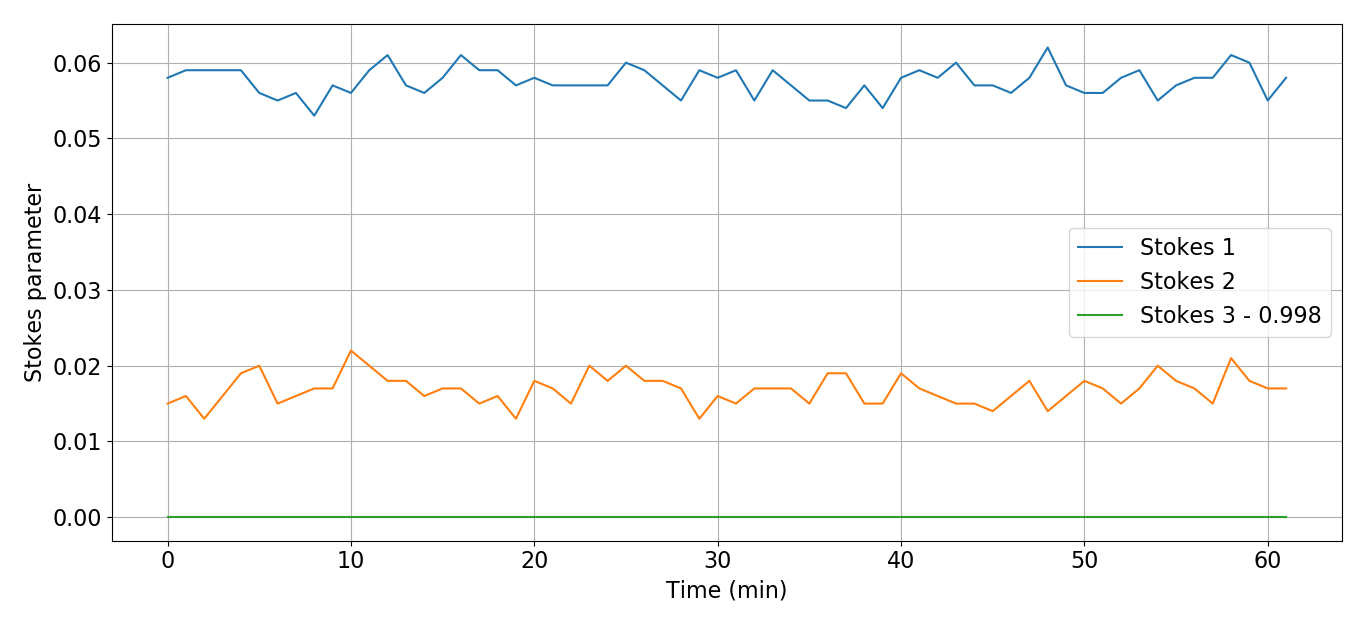
\includegraphics[width = .9\textwidth]{polstability}
\caption{Right circular polarization stability at the ion position over a period of one hour. To the third parameter $S_3$, 0.998 has been subtracted.}
\label{polstability}
\end{figure}

\begin{figure}[H]
\centering
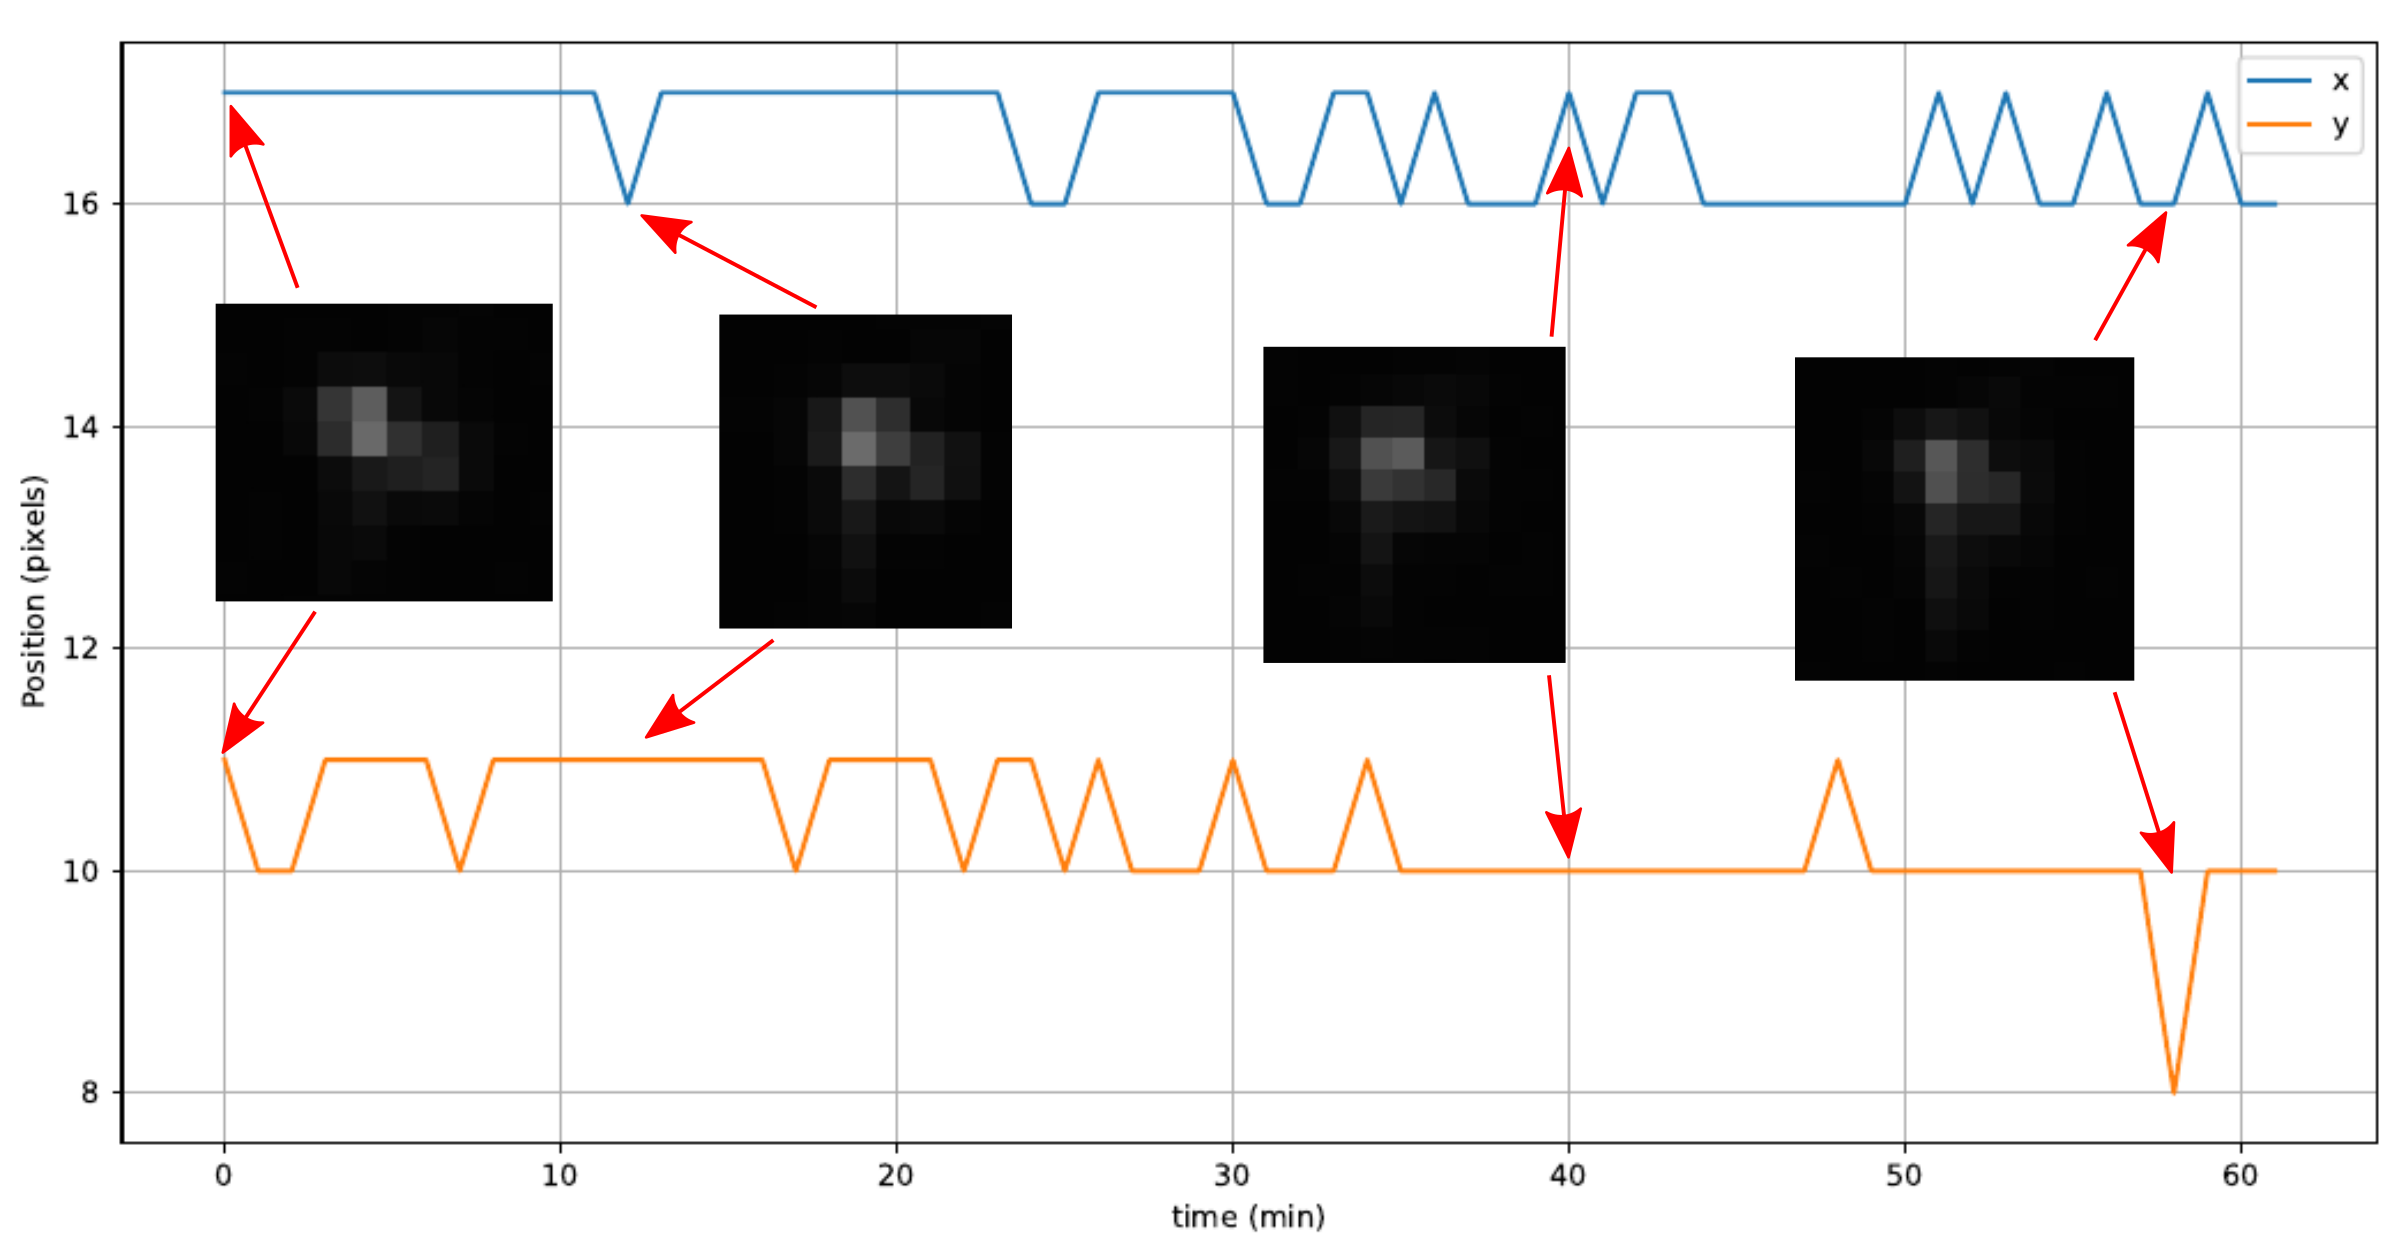
\includegraphics[width = .9\textwidth]{beampointing2}
\caption{Beam pointing stability at the focus position over a period of one hour. The 2 lines represent the horizontal $x$ and vertical $y$ position of the beam in unit of pixels. In the insets, some examples of raw data are given.}
\label{beampointing}
\end{figure}


\newpage
\section{Final installed system}
\label{sec:finalsetup}
After the tests presented in the previous sections, the setup was installed next to the ion chamber and focused on the ions as described in Section \ref{design4}. As there is no more physical access to the focus spot, more advanced quantum optics experiment have to be carried out in order to measure properties of the system, such as focus spot size and addressing error. The first experiment designed aimed at measuring these two quantities: a Ramsey experiment was performed on four loaded ions, from which the beam shape in one direction (along the ion string) due to addressed AC Stark shifts on the ions could be measured.
The second experiment involves three ions and the goal was to generate photons via Raman process from one single ion leaving the states of the other two unaltered, demonstrating therefore the new possibility to emit single photons into the cavity, from individual ions in a string.

\subsection{Single qubit manipulation}
\label{sec:singlequbitmanipulation}
\begin{figure}[H]
\centering
\includegraphics[width=\textwidth]{sequence}
\caption{Pulse sequence of the Ramsey experiment. The sequence is repeated for different AOD frequencies which moves the 3-GHz-detuned addressed 393 nm beam across the ion string. From the ion excitations, measured by the imaging CCD camera, the Rabi frequency of the 393 nm laser can be inferred. All operations are on all ions simultaneously, except the 393 nm pulse which is ideally addressed. The length $\tau$ was varying.}
\label{sequence}
\end{figure}
The goal of this experiment is to perform the Ramsey experiment discussed in Section \ref{sec:expqubit}. In summary, we want to sweep the 393 nm beam along the ion string, the sequence in Figure \ref{sequence} is repeated for different AOD frequencies, and from the ion excitation we can infer the Rabi frequency of the 393 nm laser. The Rabi frequency can then be fitted to obtain the focus spot size. Before the experiment, some preliminary measurements have to be taken, thus in this section we show first the following:
\noindent\begin{itemize}
\item Global Rabi flops with 729 nm on the qubit transition, from this we can measure the $\pi/2$ pulse time and show individual ion readout with the camera.
\item Ramsey fringes without 393 nm, showing coherent control over the ion qubits.
\item Addressed 393 nm pulse length scan, to determine the length $\tau$ of the Raman pulse to achieve particular $\sigma_z$ rotations and furthermore to estimate the addressing error.
\end{itemize}
These experiments were done with four ions loaded in the trap with endcap voltages of 714 V and 700V, for which numerical simulations yield an axial COM frequency of $\sim$767 kHz. The 393 nm laser was locked to the wavemeter and detuned from resonance by $\sim$3 GHz, ref. Section \ref{sec:expqubit}.\par
Global Rabi flops are showed in Figure \ref{rabiflops4}. Some point are missing in the plot due to a melting event of the ion crystal. The system took the data points while ions were melted, therefore they have been removed. Rabi flops are damped due to residual thermal distribution, since we only perform Doppler cooling, ions are not in the ground state, but rather in a thermal state \cite{ross}. The $\pi/2$ time is extrapolated from the first flop as the time it takes for the ions to first reach excitation probability $P_D = 0.5$, we estimated 4.2 $\mu$s. Errorbars on the excitation probability have been assigned according to the error on estimating the probability of a binomial distribution \cite{mle}
\begin{equation}
\label{errorequation}
\sigma = \sqrt{\frac{P_{D}(1-P_{D})}{N}},
\end{equation}
where $N = 50$ is the number of repetitions.
\begin{figure}
\centering
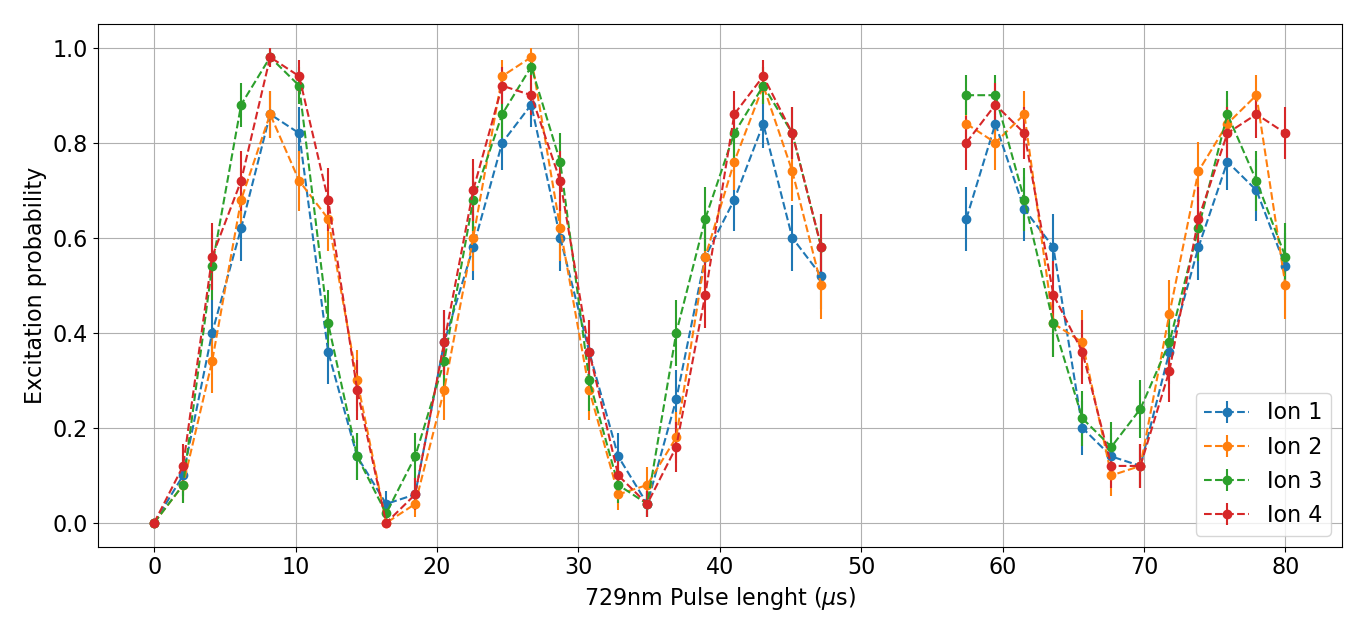
\includegraphics[width=\textwidth]{rabiflops2}
\caption{729 nm global Rabi flops on 4 ions measured with the camera. Errorbars on the excitation probability ($P_D$) have been assigned according to the error on estimating the probability of a binomial distribution. Some points were removed due to a melting event.}
\label{rabiflops4}
\end{figure}
Ramsey fringes without the 393 nm pulse are presented in Figure \ref{ramseyfringes}, the $\pi/2$ time was set to 4.2 $\mu$s. The phase $\phi$ between the two pulses was scanned, and afterwards it was set to $\phi = \pi/2$ for the rest of the experiment.
\begin{figure}
\centering
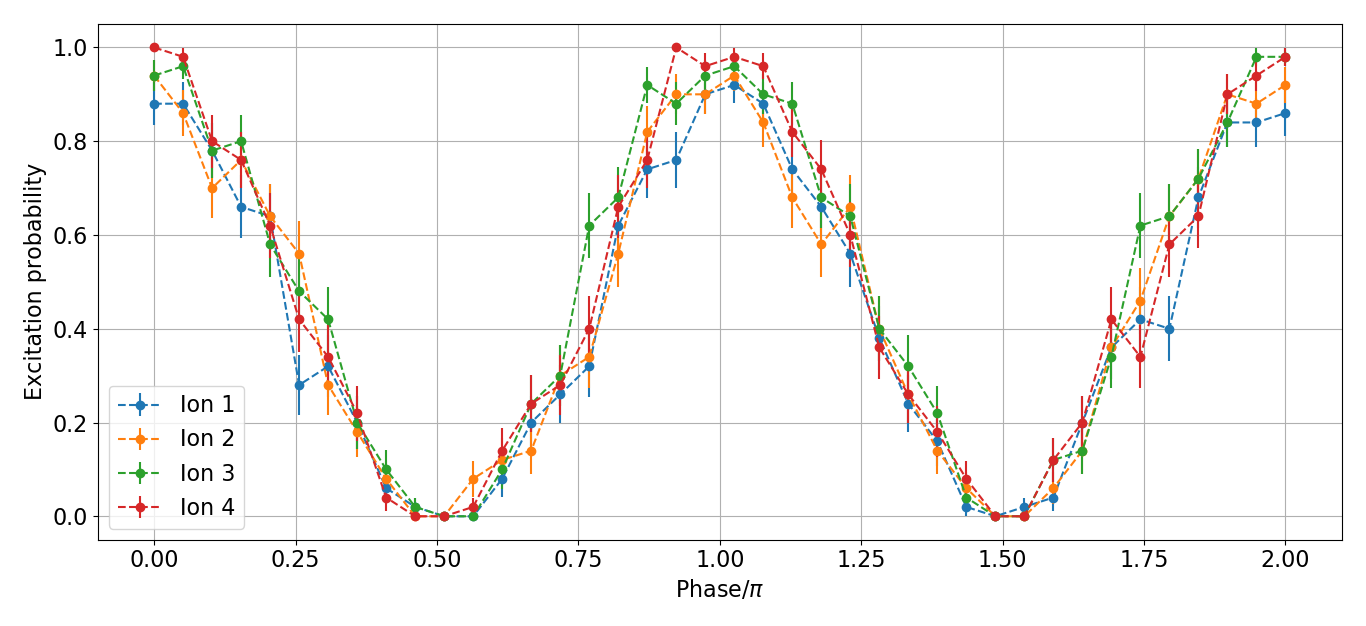
\includegraphics[width=\textwidth]{ramseyfringes}
\caption{Ramsey fringes for 4 ions without 393 nm. A $\cos^2(\phi)$ behavior can be noticed showing coherent control of the ion states.}
\label{ramseyfringes}
\end{figure}
The 393 nm pulse length $\tau$ was scanned inside the Ramsey experiment, the flops are showed in Figure \ref{ACscan}. For the next experiment, to get the beam profile across the ion string, we chose $\tau$ of 25 $\mu$s, so that the ion is not fully flipped. It was roughly checked that $\tau$ is the same for every ion.
\begin{figure}
\centering
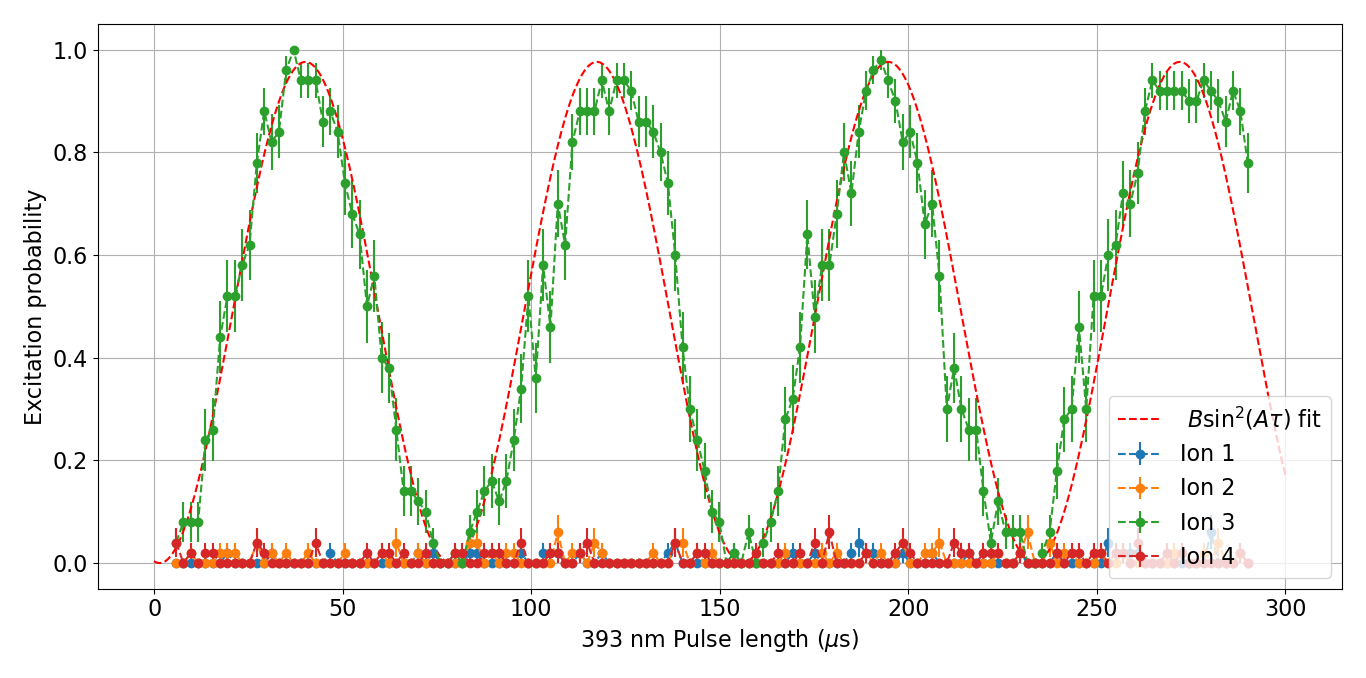
\includegraphics[width=\textwidth]{ac_stark_fit2}
\caption{393 nm AC Stark flops. The pulse length $\tau$ of the 393 nm laser is scanned while shining over one singe ion. The red curve is a fit of $B\sin^2(A\tau)$, where $A$ is proportional to the Rabi frequency of the laser focused on the third ion.}
\label{ACscan}
\end{figure}
Finally, the AOD frequency is scanned, during this scan the beam is moved from ion to ion, for each beam position, the excitation probability of all ions is measured, this is then translated to Rabi frequency with Equation \eqref{eq:ptointensity}. The result after further post analysis can be seen in Figure \ref{AODscan}. Specifically, the square of the Rabi frequency, determined from the probability $P_D$, gives the laser intensity of the beam.
\begin{figure}
\centering
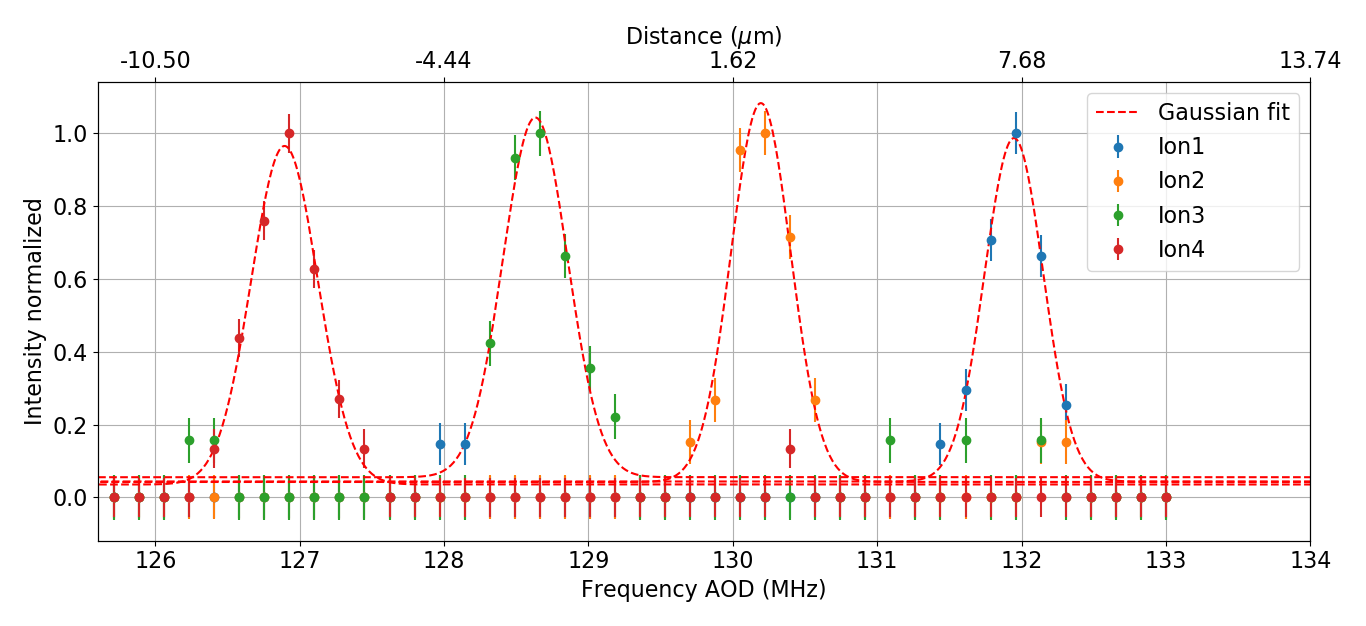
\includegraphics[width=\textwidth]{img/AODScan}
\caption{AOD scanning of four ions via Ramsey interferometry. The normalized intensity comes from the Rabi frequency calculated from the measured excitation probability $P_D$ using formula \eqref{eq:ptointensity}. The upper micrometer scale is calibrate by comparing the center of the Gaussian fit with the numerically calculated ion positions.}
\label{AODscan}
\end{figure}
To calibrate the beam position scale in micrometers, the axial COM mode (767 kHz) of the trap is measured by performing 729 nm spectroscopy on the carrier and motional sideband. Ions positions can be then numerically calculated (cfr. Section \ref{ionstrings}). AOD frequencies corresponding to the maxima in Figure \ref{AODscan} are attributed to the ion positions, and corresponding frequency shifts to distances. By comparison, we found a conversion factor of $3.03\,\mu\text{m}/\text{MHz}$.
The four peaks have been fitted with a Gaussian function to obtain the waist of the beam when focused on the different ions. The waists yielded by the fits are from right to left $\omega_1 = 1.23\pm 0.20\,\mu$m, $\omega_2 = 1.25\pm 0.19\,\mu$m, $ \omega_3 = 1.35\pm 0.22\,\mu$m, $\omega_4 = 1.39\pm 0.20\,\mu$m.\par
Figure \ref{ACscan} allows the addressing error, when aiming at ion 3, to be determined. In this measurement, the addressing beam was focused on one ion and the Raman length $\tau$ is scanned. This increases the interaction time of the laser with the ions, and if the interaction is long enough even the tail of a Gaussian can induce some excitation on the ions on the side of the one being addressed. In the scan displayed, the pulse reached 300 $\mu$s and there is no statistically significant excitation on any ion apart from the one flopping. Others scans went up to 500 $\mu$s, and still no visual excitation is present. While this means that no quantitative number can be determined for the addressing error, an upper bound can still be given. A sinusoidal fit $B\sin^2(A\tau)$ has been done on the data, it is not perfect probably due to intensity fluctuations of the lasers, or magnetic field fluctuations. Nonetheless, from the fit we can determine the Rabi frequency on the third ion as $\Omega_3 = \sqrt{4\Delta \cdot A} = 22\,\text{MHz}$, see Equation \eqref{stupidequation}. Assuming in the worst case scenario that an excitation $P_D>0.05$ on the second ion appears right after 500 $\mu$s, i.e. the Rabi frequency of the non-addressed ion is $2$ MHz, the addressing error should be at most $\Omega_2^2/\Omega_3^2< 10^{-2}$.\par
During this experiment we scanned the AOD twice with an interval of 30 minutes to measure the stability of the system. In Figure \ref{fig:stability} the peak on the third ion has been overlapped between the two scans. A fit gives the central frequencies of the two peaks, and their difference determines the stability over a period of 30 minutes, we estimated a stability of $0.20\pm 0.07\,\mu$m/hr.\par
To conclude, we remark that in the presented experiments in this section the 393 nm pulse acts as a single qubit gate on individual ions. The Ramsey experiment carried out by scanning the AOD frequency demonstrated the ability of the system to manipulate single qubits as it includes a single qubit rotation $\sigma_z$ first introduced in Section \ref{sec:quantumoperations}. The Ramsey experiment therefore fulfills Goal 2 of this thesis, however the gate quality of $\sigma_z$ needs to be studied more carefully in the future.
\begin{figure}
\centering
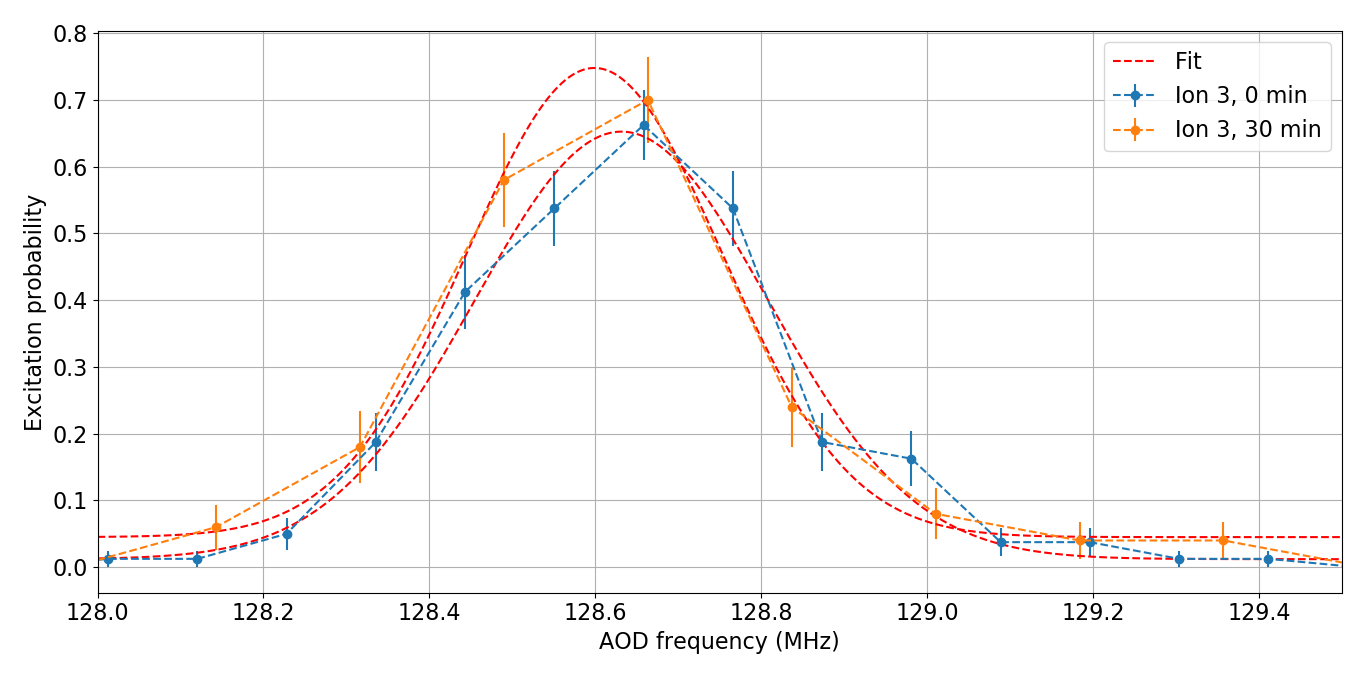
\includegraphics[width=\textwidth]{stability}
\caption{AOD scanning on one single ion repeated after 30 minutes to measure stability as difference of the center of the two peaks: $0.20\pm 0.07\,\mu$m/h. Processing of the data has been done as in Figure \ref{AODscan}.}
\label{fig:stability}
\end{figure}
\subsection{Photon production}
\label{exp:photons}
The second thesis goal is to generate single cavity photons from individual ions in a chain. Photons are produced by a pulse of 393 nm light focused on the central ion of three via the cavity-mediated Raman process described in Section \ref{sec:expphoton}. The length of the Raman pulse is scanned and the integrated photon detection probability is recorded, measured leaving the cavity. The generated photon is emitted into the cavity, transmitted through the output mirror of the cavity, coupled into an optical fiber, and passes through waveplates and a PBS before reaching a superconducting nanowire single-photon detector (SNSPD)\footnote{Scontel SNSPD model FCOPRS-CCR, 854 nm detectors: $\sim 87$\% efficiency, $\sim 0.5$ dark counts per second.}. In contrast to the previous experiment where the 393 nm laser is used to impart an AC Stark shift, here the precise (to the kHz level) frequency of the Raman laser is key to generating cavity photons (the cavity has a linewidth of $\sim$70 kHz and the laser should be significantly less for efficient photon generation). Therefore, to generate photons, the 393 nm laser is locked to an external cavity (linewidth $\sim$100 Hz Ref. \cite{helene}). The existing AOM network was established to leave the Raman laser 400 MHz detuned from the S-P transition. To account for the additional 127 MHz detuning of the AOD, we shifted the frequency of two AOMs in the 393 nm setup (see Section \ref{sec:393setup}).\par
%The experiment was carried out in a single day at the end of the time available for my master work.
We loaded three ions in the trap with a measured axial COM frequency of $\sim 820$ kHz, which means ion separations of 5.4 $\mu$m. We locked the 393 nm laser to the cavity and scanned the frequency with the double pass AOM 1 (ref. Figure \ref{scheme393}). The transition chosen is $\ket{S_{1/2},-\frac{1}{2}}\to \ket{D_{5/2},-\frac{3}{2}}$, see details in Section \ref{sec:expphoton}. The cavity position along its principal axis was optimized using a piezo in order to maximize overall 854 nm photon count rate when driving the Raman process with the addressed beam aligned to the central ion, and simultaneously repumping the 854 nm transition (so multiple photons can be generated to enhanced the signal). Assuming that the central ion is at a maximum of the cavity field and that the cavity-trap angle is $4.6^\circ$, we calculated that the two outer ions are at 82 \% of the cavity maximum.
In the experiment we included an initial stage of Doppler cooling and a final stage of ion qubit-state detection with the camera. Furthermore, the 806 nm cavity locking light was switched off during the photon generation process, in this time the cavity maintained its position with a sample and hold. For each Raman pulse length, the experiment is repeated $N=200$ times to get an estimate for the average photon probability and the ion excitation probability ($P_D$ the probability to find the ion in the D5/2 manifold). Errorbars on the excitation probability are calculated as in the previous section (Equation \eqref{errorequation}), while for the photon probability the error is modelled by Poissonian statistics \cite{quantumoptics}
\begin{equation}
\sigma_{ph} = \frac{\sqrt{N_{click}}}{N},
\end{equation}
where $N_{click}$ is the number of times a photon has been detected with respect to the total $N$ repetitions. \par
The experiment consisted of scanning the Raman pulse length, and for each length, the photon detection probability and the ion excitation probability $P_D$ have been measured. In Figure \ref{probphoton}, the photon detection probability is plotted. From polarization selection rules, we expect a $\pi$ polarized photon to be emitted. As the cavity is perpendicular to the magnetic field, the photon in the cavity is linearly polarized and is then rotated with waveplates such that it goes to one output port of the PBS. Consistent with the expectations, we can see that we measured mostly vertical polarized photons. The photons are not perfectly polarized which could be due to imperfections of the polarization analysis, e.g. errors in the settings of waveplates.\par
The excitation probability $P_D$ is plotted in Figure \ref{probion}. In this figure, we can see that only the addressed ion is excited to the $\text{D}_{5/2}$ state, while the others show no excitation at all. $P_D$ does not reach 1, perfect population transfer is not achieved due to non-zero spontaneous emission from the $\text{P}_{3/2}$ state to the $\text{D}_{3/2}$ state, or to the $\ket{S_{1/2},+\frac{1}{2}}$ state. Unfortunately, we were not able to simulate theoretical curves for both of the plots, as the experiment was carried out in one day at the end of the time available for my master work. As such, no careful optimization was done on the polarization of the driving addressing beam, which means that the parameters (specifically, the Rabi frequency of the addressed laser) are not well known enough do a theoretical model. We remind that the two outer ions are still coupled to the cavity to a significant extent (82\% coupling expected) such that they are in a condition to generate photons if the addressed beam were to drive them. In fact, we also observed photon generations when addressing outer ions.\par
In conclusion, we observed the addressed ion getting excited to the $\text{D}_{5/2}$ state and simultaneously detected vertical polarized photons. Therefore, these data are consistent with only the addressed ion emitting a cavity photons.
\begin{figure}
\centering
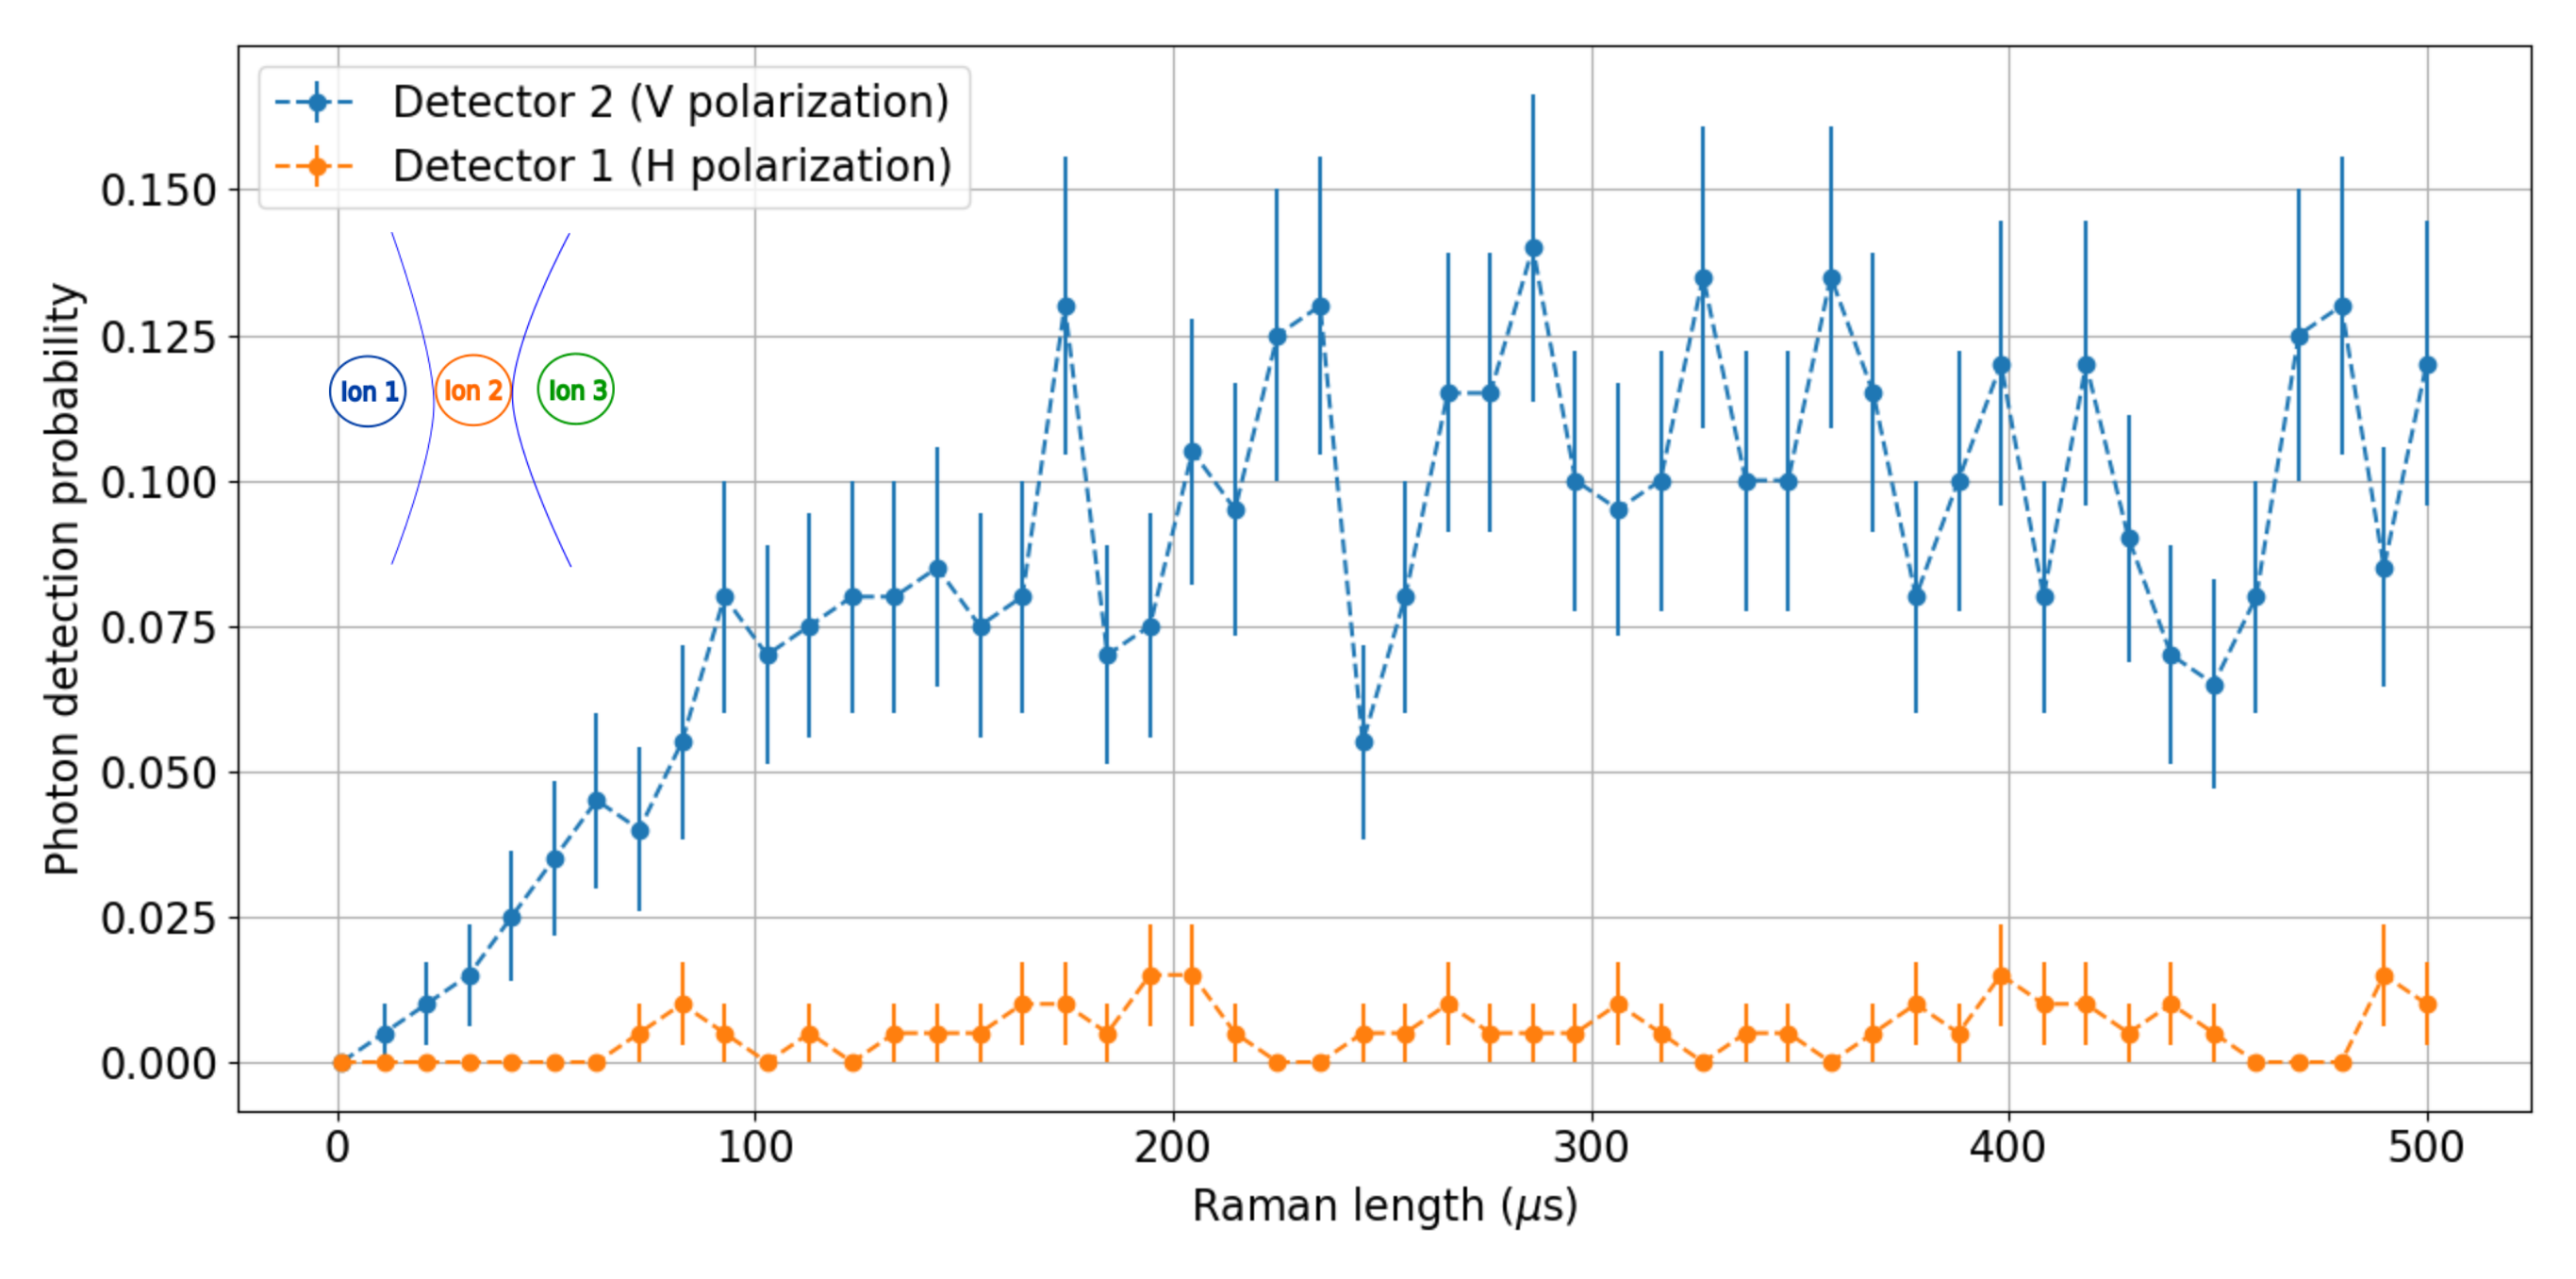
\includegraphics[width=\textwidth]{img/photonefficency_witherror3}
\caption{Measured cavity photon detection probability as a function of addressed Raman laser pulse length. The two detectors measure the Horizontal (orage data points) and Vertical (blue data points) photons emitted by the ion, in Figure \ref{probion} excitations of the ions during the process are plotted. Inset: diagram of the situation where only the middle ion is addressed.}
\label{probphoton}
\end{figure}
\begin{figure}
\centering
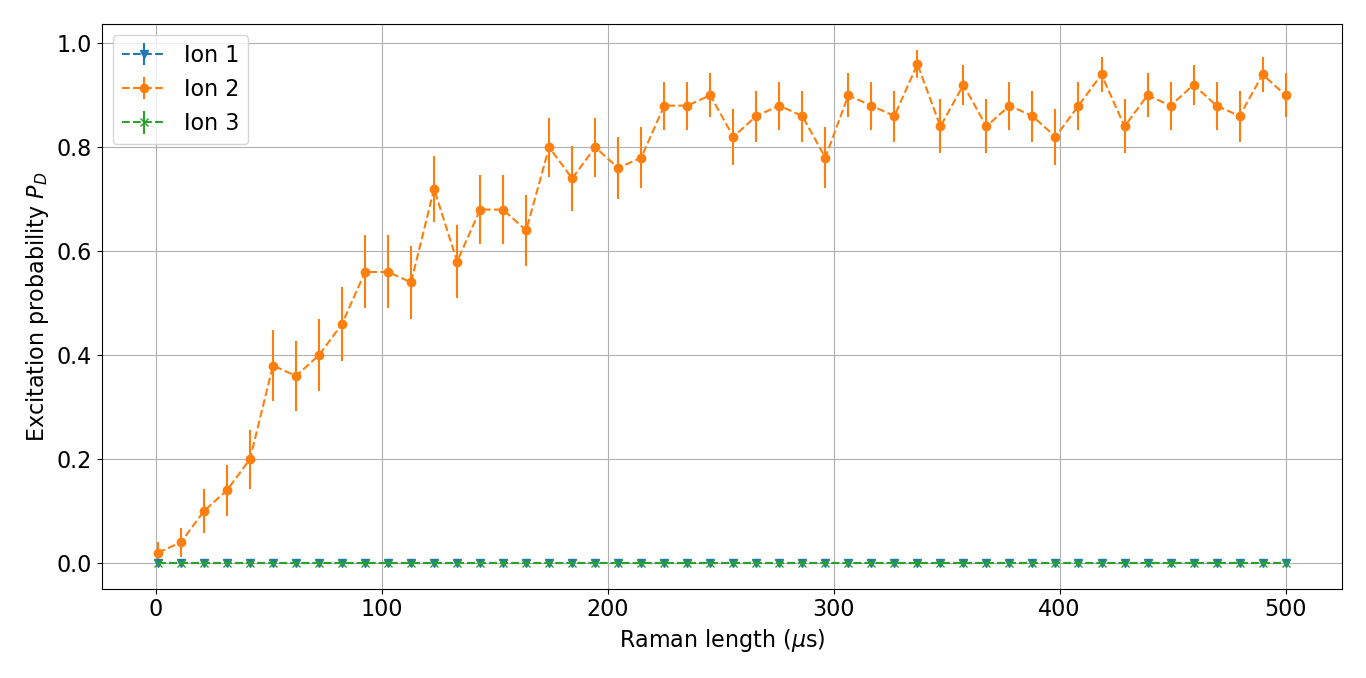
\includegraphics[width=\textwidth]{img/ramanlength_witherrors2}
\caption{Qubit excitation state of the ions $P_D$ as a function of addressed Raman laser pulse length. In Figure \ref{probphoton} photon detection probability during the same experiment is plotted.}
\label{probion}
\end{figure}
% \section{Final properties summary}
% This section contains a summary of the different properties of the setup, everything can be found in the figure below.
% \begin{figure}[H]
% \centering
% \includegraphics[width = \textwidth]{recap}
% \caption{Properties summary of the setup.}
% \end{figure}
